\subsection{Server und Hosting-Details}
Unsere Website wird auf einem vServer (VPS) gehostet, der bei noez.de angemietet ist. Dies bietet uns eine kostengünstige, aber leistungsfähige Lösung für das Hosting mit umfangreichen Konfigurationsmöglichkeiten. Die Primär-IP unseres Servers lautet 5.231.1.40, und wir haben umfassenden Zugriff auf das Servermanagement über ein benutzerfreundliches Webinterface.

\subsubsection{Technische Spezifikationen}
Der Server wird von einem Linux Ubuntu System betrieben und verfügt über 1020.05 MB RAM und eine CPU-Auslastung, die selten 0.08\% überschreitet, was auf eine effiziente Nutzung der Ressourcen hinweist. Der Trafficverbrauch liegt bei 8.06 GB von einem verfügbaren Volumen von 1000 GB pro Monat, was darauf hindeutet, dass wir gut innerhalb unserer Kapazitätsgrenzen operieren.

\subsubsection{Skalierbarkeit und Zugriffsmanagement}
Einer der Hauptvorteile unseres VPS ist die problemlose Skalierbarkeit. Durch einfaches Upgraden auf einen besseren Plan können wir die Serverressourcen je nach Bedarf erhöhen. Der volle Zugriff auf den Server mit Root-Rechten ermöglicht es uns, jederzeit Anpassungen vorzunehmen oder zusätzliche Dienste zu integrieren. Die Verwaltung des Servers erfolgt durch einen dedizierten Account, der ausschließlich von einer dafür spezialisierten Person unseres Teams gehandhabt wird.

\subsubsection{Sicherheit und Monitoring}
Die Details zu den Sicherheitsvorkehrungen und dem Monitoring unseres Servers sind in Abschnitt 5.8.2 des Berichts ausführlich dargestellt. Dort werden die Maßnahmen beschrieben, die nach einem Sicherheitsvorfall ergriffen wurden, einschließlich der verstärkten Sicherheitsprotokolle und der Nutzung von Fail2Ban.

\subsubsection{SEO und Google Analytics}
Die Nutzung unseres Servers ermöglicht auch die effektive Implementierung von SEO-Strategien und die Integration von Google Analytics. Diese Tools sind essenziell, um die Sichtbarkeit unserer Website zu erhöhen und detaillierte Einblicke in das Verhalten der Besucher zu erhalten. Weitere Informationen hierzu finden sich in Abschnitt 5.7.5 des Berichts.

\begin{figure}[h]
\centering
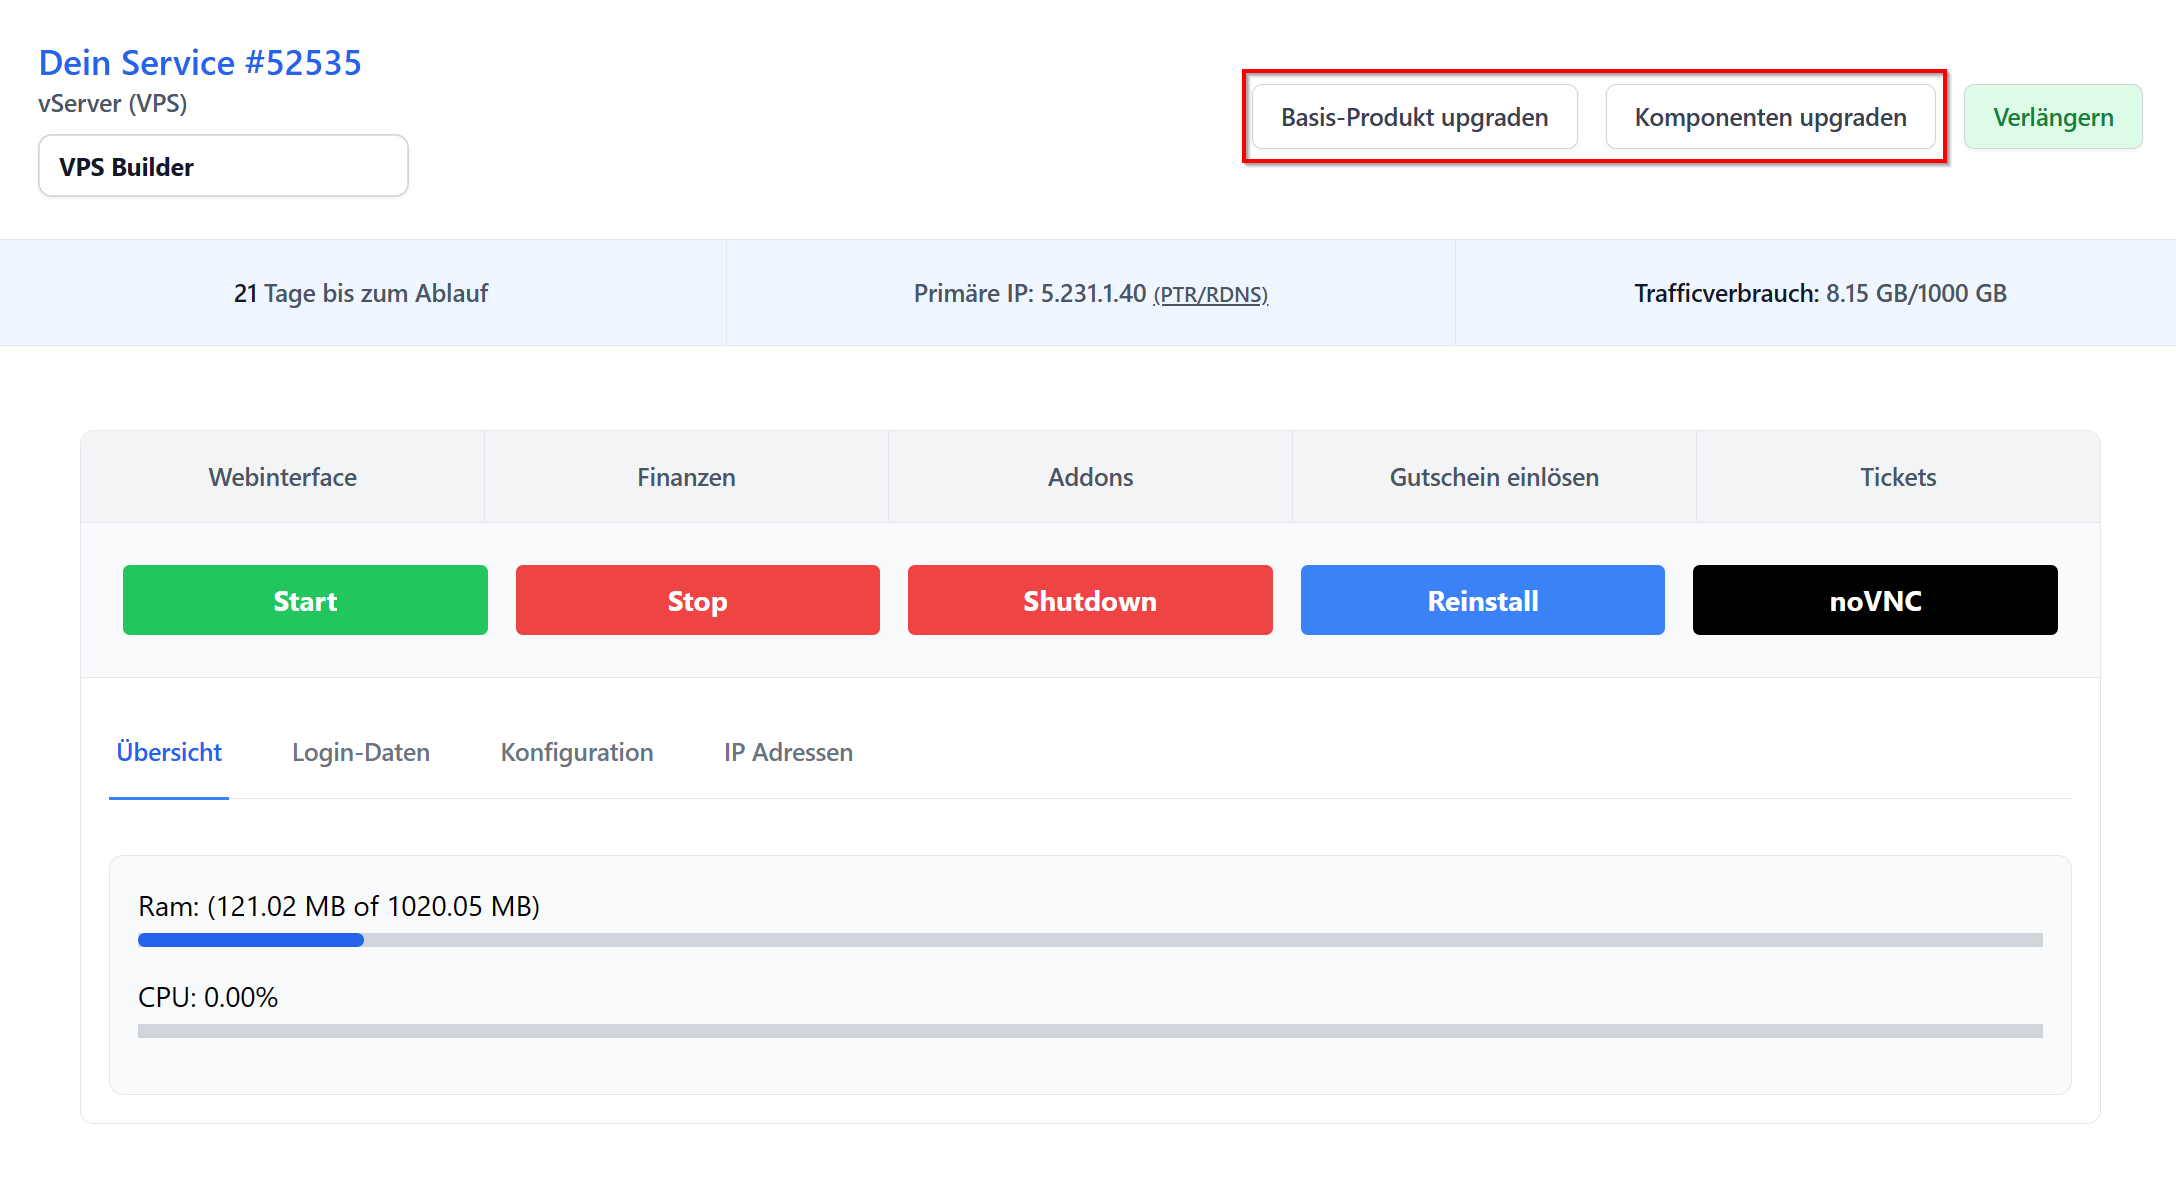
\includegraphics[width=1\textwidth]{Resources/hosting.png}
\caption{Screenshot des Server-Dashboards, der die Übersicht und Kontrolle des Hostings visualisiert.}
\end{figure}

Die robuste und flexible Hosting-Lösung stellt sicher, dass unsere Website nicht nur zuverlässig läuft, sondern auch gut auf zukünftiges Wachstum und zusätzliche Anforderungen vorbereitet ist.
